\documentclass{article}
\usepackage[frenchb]{babel}
\usepackage[utf8]{inputenc}
\usepackage[T1]{fontenc}
\usepackage{graphicx}
\usepackage{fancyhdr}
\usepackage{float}

\pagestyle{fancy}
\title{Projet de Programmation par Contraintes : Élisabeth}
\author{T.Béziers La Fosse, D.Bordet, J. Clayton, A. Giraudet, B. Moreau}




\begin{document}

\renewcommand{\contentsname}{Sommaire} 


\maketitle
\date


\begin{figure}[h]

\begin{center}
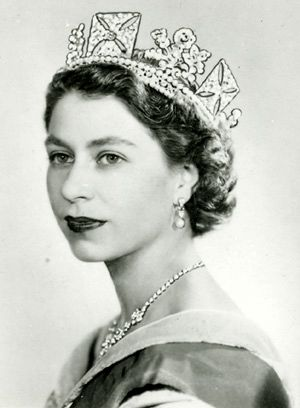
\includegraphics[width = 250px]{./picture/eli.jpg}
\end{center}

\end{figure}




\newpage

\tableofcontents

\newpage

\section{Introduction}

\vspace{1cm}

\subsection{Problématique et but du projet}

\vspace{1cm}

Dans le cadre du module de Programmation par Contraintes en Master 1 ALMA, nous avons eu pour objectif d'implémenter un solveur capable de résoudre le problème des \emph{N-Queens}. 

Ce projet est étendu sur trois séances, durant lesquelles nous avons dû concevoir ce solveur, capable d'effectuer une recherche complète des solutions, mais aussi une recherche locale, et enfin comparer les résultats d'exécutions sur des problèmes de taille variable.

Pour implémenter notre solveur, nous avons pris la décision d'utiliser le langage de Programmation Python3. Nous avons hésité avec $C++$, mais avons finalement choisi ce premier. Même si ses performances sont légèrement moins bonnes qu'avec $C++$, nous apprécions sa simplicité d’utilisation. De plus aucun autre module de notre Master ne nous a donné l’occasion de nous en servir, si bien que nous avons vu ici une opportunité pour nous réhabituer à ce langage particulièrement au goût du jour.

Dans ce rapport nous verrons en première partie le problème des \emph{N-Queens} avec plus de précision. Ensuite nous parlerons de la recherche complète que nous avons implémenté, puis la recherche locale. Enfin nous comparerons nous résultats d'exécution. 


\vspace{1cm}

\subsection{Problème des N-Queens}

Le problème des \emph{N-Queens} est un problème très célèbre dans le monde des mathématiques. Ce problème posé pour la première fois en 1850 par Franz Nauck consiste à trouver poser $n$ reines sur un échiquier faisant $n$ cases de côté sans qu'elles puissent s'attaquer. Ainsi elles ne doivent pas: 
\begin{itemize}
\item Etre sur la même ligne
\item Etre sur la même colonne
\item Etre sur la même diagonale
\end{itemize}

Ce problème pose quelques problèmes, car il n'existe pas d'algorithme polynomial en complexité.


En testant toutes les possibilités de placement des reines sur un échiquier de taille $8*8$ avec un algorithme de recherche exhaustive, on se retrouve à parcourir $64^8$ placements possibles, soit $2^{48}$, si bien qu'on arrive rapidement à des temps d'exécution bien trop longs. Néanmoins on peut réduire facilement ce temps d'exécution avec la programmation par contraintes. 


\subsubsection{Contraintes}

On doit ainsi modéliser les contraintes dans notre programme pour réduire drastiquement le nombre d'itérations avant de trouver une solution. Les contraintes, en langage naturel, sont donc:

\begin{itemize}
\item Il doit y avoir qu'une reine par ligne.
\item Il doit y avoir qu'une reine par colonne.
\item Il ne doit pas y avoir plus d'une reine par diagonale;
\end{itemize}

Ainsi pour modéliser ceci sous la forme d'un CSP, on utilisera les variables suivantes:
$x_i$: Reine de la ligne $i$.
$x_i = j$ : $j$, numéro de la colonne où est placée la reine.

Avec ce modèle on est sûr qu'il n'y aura pas d'attaques si deux reines sont sur la même ligne, puisqu'on ne permet qu'une seule reine par ligne.
Les contraintes sont donc les suivantes:
\begin{itemize}
\item Pas d'attaque sur les colonnes: $allDifferent(x_i)$ $\forall i \in [1, n]$. $\forall i \neq j$, $x_i \neq x_j$

\item Pas d'attaque sur les diagonales:  $\forall i \neq j, |x_i - x_j| \neq |i - j|$, et $\forall  1 \leq i < j \leq n : |x_i - x_j | \neq j - i$
\end{itemize}


\section{Complete Search}

La recherche complète consiste à trouver toutes les solutions d'un problème, ou bien à prouver qu'il n'existe pas de solutions. 
Pour effectuer cette recherche complète on utilise un algorithme de \emph{Branch \& Prune}, celui vu en cours. 

On part d'un nœud vide, et pour chaque possibilité d'assignement de la variable suivante on crée une branche, c'est le \emph{branching}.

On assigne donc nos variables $x_i$ une par une et on retire les valeurs qui ne valident pas les contraintes du domaine des variables pour les branches suivantes, c'est le \emph{pruning}. S'il n'y a plus de valeur possible dans le domaine d'une variable, c'est que l'assignement ne valide pas les contraintes. On peut donc fermer la branche et passer à la suivante.

Ainsi toutes les branches dans lesquelles toutes les variables sont assignées sont une solution. Et de cette manière, en récupérant tous ces assignements différents, on a autant de solutions pour notre problème. 

\clearpage

Dans l'exemple suivant, on assigne la variable montrée par la croix. Lors de notre pruning, on réduit donc du domaine des variables suivantes toutes les cases grisées, c'est à dire les cases sur la même colonne, et sur les diagonales, qui violent les contraintes. 
https://thewalnut.io/app/release/11/ 
\begin{figure}[h]
\caption{\label{reine1} Première Reine}
\begin{center}
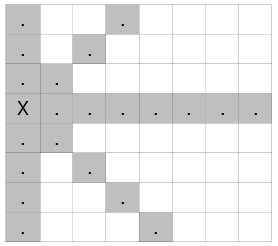
\includegraphics[scale=0.5]{./picture/pruning1.png}
\end{center}
\end{figure}

On assigne ensuite une seconde variable, et on recommence tant que le domaine de la variable suivante n'est pas vide. Auquel cas la branche ne peut aboutir à une solution et on l'abandonne.

\begin{figure}[h]
\caption{\label{reine2} Seconde Reine}
\begin{center}
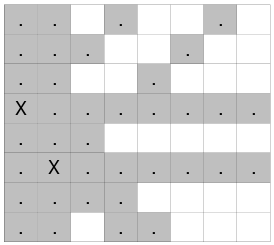
\includegraphics[scale=0.5]{./picture/pruning2.png}
\end{center}
\end{figure}

Ainsi on peut trouver toutes les solutions possibles au problème des NQueens.


\section{Local Search}

La recherche locale de notre programme, par rapport à la recherche complète, s'arrête dès qu'elle trouve une solution au problème. L'algorithme implémenté se nomme
\emph{min-conflicts algorithm}. 

Pour trouver une solution, l'algorithme numérote chaque cellule de la ligne courante par le nombre de collision avec d'autres reines. C'est-à-dire, si une cellule se trouve sur la même ligne qu'une autre reine, La cellule a 1 pour valeur. Si elle est en plus à la diagonale d'une seconde reine, elle a 2 comme valeur.
Ainsi pour placer nos reines, on choisira toujours les cases valant 0.

Lorsque plusieurs cellules de la ligne courante ont 0 comme valeur, on choisira la première parcourue. On aurait pu aussi la choisir de manière aléatoire, mais afin d'améliorer le temps d'exécution c'est la première solution que nous avons choisi. 


\begin{figure}[!h]
	\caption{\label{local1} Échiquier vide}
	\begin{center}
	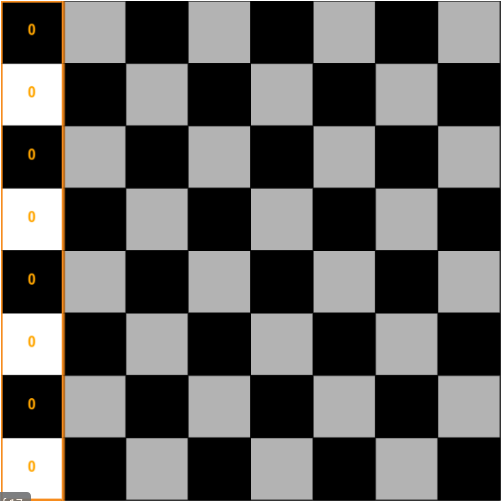
\includegraphics[scale=0.3]{./picture/local1.png}
	\end{center}
\end{figure}

Ainsi on commence par la première ligne, en ayant 0 comme valeur sur chaque cellule. 

\clearpage
\begin{figure}[!h]
	\caption{\label{local2} Premier parcours}
	\begin{center}
	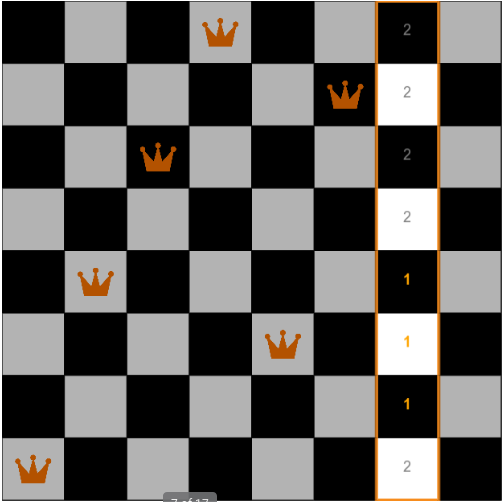
\includegraphics[scale=0.3]{./picture/local2.png}
	\end{center}
\end{figure}

On place la première reine arbitrairement, on calcule ensuite l'indice de chaque cellule des lignes suivantes, jusqu'à avoir placé une reine sur chaque ligne. Si une ligne ne comporte pas de cellule indicée à 0, dans ce cas on place la reine sur l'indice minimum. 

\begin{figure}[!h]
	\caption{\label{local3} Retour en arrière}
	\begin{center}
	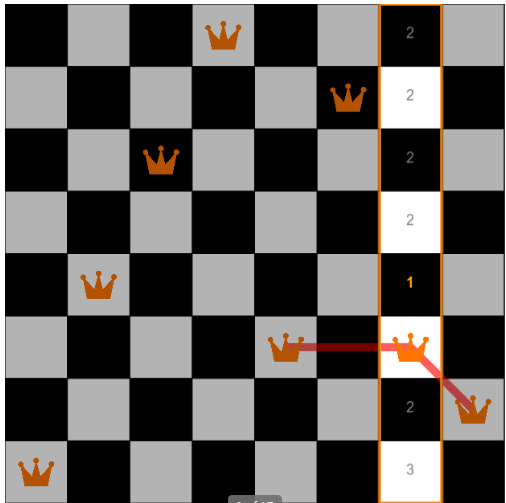
\includegraphics[scale=0.3]{./picture/local3.png}
	\end{center}
\end{figure}

Enfin, lorsque la reine de la dernière ligne a été placée, on se rend sur la reine violant une contrainte la plus proche. On la déplace sur la cellule de la ligne qui a l'indice minimum. Si cette cellule n'est pas à 0, c'est qu'une nouvelle reine viole une contrainte, on se rend à nouveau sur cette reine, et on la déplace. On recommence tant que des contraintes sont violées. 

\section{Résultats d'exécution}
\subsection{Complete search}
\begin{figure}[!h]
	\caption{\label{csearch} Recherche complète}
	\begin{center}
	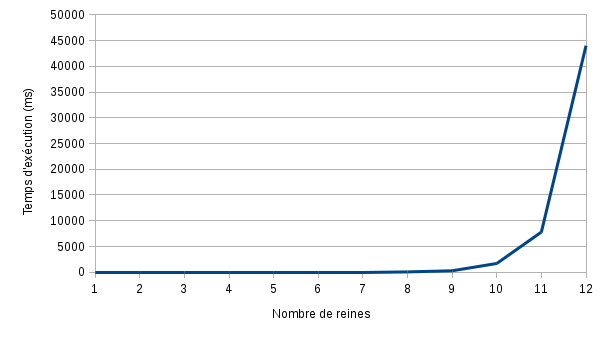
\includegraphics[scale=0.5]{./picture/compelte_search.png}
	\end{center}
\end{figure}
Voici les résultats d'exécution de l'algorithme de recherche complète de solutions. On voit assez rapidement que le temps d'exécution croit de manière exponentielle, puisque à partir de 12 reines, l'exécution dure 44 secondes. Nous n'avons pas fait plus d'exécutions pour une raison évidente de temps d'exécution.

\subsection{Local search}
\begin{figure}[!h]
	\caption{\label{lsearch} Recherche locale}
	\begin{center}
	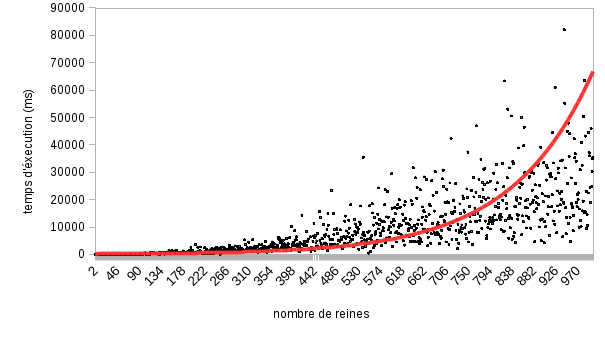
\includegraphics[scale=0.5]{./picture/local_search.png}
	\end{center}
\end{figure}
Voici ici les résultats d'exécution de l'algorithme de recherche locale d'une solution. Par rapport à l'algorithme précédent, on peut aller bien plus loin dans le nombre de reines. La croissance est elle aussi exponentielle, mais permet des résultats bien plus rapides qu'avec une recherche complète. 

\section{Conclusion}
Pour conclure ce projet, l'implémentation des algorithmes de recherche de solutions a été un exercice très intéressant, et nous a notamment permis de comprendre beaucoup plus aisément les algorithmes vus en cours. En voyant les résultats d'exécution, on comprend rapidement que l'algorithme de recherche locale est bien plus rapide que celui de recherche complète. Si bien qu'il vaut mieux utiliser ce dernier dans le cas où on a besoin de toutes les solutions. Ainsi l'algorithme de recherche locale est plutôt efficace dans le cadre d'un problème de satisfiabilité. blabla
\section{Sources}

\begin{tabular}{|c|c|}
\hline
Image & Source \\
\hline
\ref{reine1} & http://www.cs.cornell.edu/~wdtseng/icpc/notes/bt2.pdf \\
\ref{reine2} &  \\
\hline
\ref{local1} & \\
\ref{local2} &  https://thewalnut.io/app/release/11/ \\
\ref{local3} &  \\
\hline
\end{tabular}

% \lfoot{\small{Source: http://www.cs.cornell.edu/~wdtseng/icpc/notes/bt2.pdf}}

\end{document}
